\documentclass[11pt]{article}
\usepackage[margin=1in]{geometry}
\usepackage{amsmath,amssymb,amsthm}
\usepackage{microtype}
\usepackage{tikz}
\usetikzlibrary{calc}
\usepackage{parskip} % nice paragraph spacing for prose
\usepackage{hyperref}

\title{Count the triangles in a five-sided star}
\author{Souvik Sarkar \\ \texttt{sounix000@gmail.com}}
\date{February 9, 2026}

\begin{document}
\maketitle

\section*{Problem}
Count the number of distinct triangles formed when a regular pentagram is drawn inside a regular pentagon by connecting every second vertex (i.e., draw the five-pointed star formed by skipping one vertex each time).

% --- Crisp TikZ figure, no labels, no caption ---
\begin{center}
  \vspace{0.5em}
  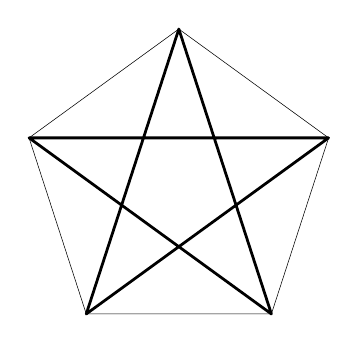
\begin{tikzpicture}[line join=round, line cap=round, x=1cm, y=1cm, scale=1]
    % Parameters
    \def\r{2.0}          % outer radius of pentagon
    \def\ang{90}         % starting angle so top vertex at 90 degrees

    % compute outer 5 vertices
    \foreach \i in {0,...,4} {
      \coordinate (V\i) at ({\ang - 72*\i}:\r);
    }

    % draw outer pentagon (thin)
    \draw[very thin] (V0) -- (V1) -- (V2) -- (V3) -- (V4) -- cycle;

    % draw pentagram (thicker)
    % connect every second vertex: V0->V2->V4->V1->V3->V0
    \draw[line width=1pt] (V0) -- (V2) -- (V4) -- (V1) -- (V3) -- cycle;
  \end{tikzpicture}
  \vspace{0.5em}
\end{center}

\section*{Strategy}
Outline of the counting method:

\begin{itemize}
  \item Classify triangles by the types of their vertices: whether a vertex lies on the outer pentagon (``perimeter vertex'') or at an intersection point formed by the pentagram (``internal point'').
  \item Use the $5$-fold rotational symmetry to count representatives of each class and multiply appropriately; verify there is no double counting.
  \item Where necessary, examine local configurations around one vertex/edge and propagate by symmetry.
\end{itemize}

\section*{Solution}
We proceed by enumerating triangle types.

\paragraph{Type I: three perimeter vertices.}
Choose any $3$ of the $5$ outer vertices. This gives
\[
\binom{5}{3}=10
\]
triangles.

\paragraph{Type II: two perimeter vertices and one internal intersection.}
Consider an outer edge as a potential base. For each outer edge there are a fixed finite number of internal intersection points that together with that base produce triangles contained in the figure. A local inspection (or symmetry argument) shows there are $3$ distinct interior-point choices per edge that yield distinct internal triangles, and counting over the $5$ edges gives
\[
5\times 3 = 15
\]
triangles of this type.

\paragraph{Type III: one perimeter vertex and two internal intersections.}
Around each outer vertex, the two nearby intersection points formed by the star lines create exactly one triangle together with that vertex (by symmetry and direct inspection). Hence there are
\[
5
\]
triangles of this type.

\paragraph{Type IV: three internal intersection points.}
Some triangles are formed solely by three intersection points of the star's diagonals. By symmetry and explicit counting of admissible intersection-triples one finds
\[
5
\]
such triangles.

\medskip
\begin{center}
\fbox{%
\begin{minipage}{0.95\linewidth}
Summing the above counts yields the total number of distinct triangles formed:
\[
10 + 15 + 5 + 5 = 35.
\]
\end{minipage}%
}
\end{center}

\section*{Conclusion}
By classifying triangles according to vertex types and exploiting the pentagon's symmetry, one deduces that the pentagon with its inscribed pentagram contains exactly $\mathbf{35}$ distinct triangles.

\end{document}
